%===============================================================================
% LaTeX sjabloon voor de bachelorproef toegepaste informatica aan HOGENT
% Meer info op https://github.com/HoGentTIN/latex-hogent-report
%===============================================================================

\documentclass[dutch,dit,thesis]{hogentreport}

% TODO:
% - If necessary, replace the option `dit`' with your own department!
%   Valid entries are dbo, dbt, dgz, dit, dlo, dog, dsa, soa
% - If you write your thesis in English (remark: only possible after getting
%   explicit approval!), remove the option "dutch," or replace with "english".

\usepackage{lipsum} % For blind text, can be removed after adding actual content

%% Pictures to include in the text can be put in the graphics/ folder
\graphicspath{{../graphics/}}

%% For source code highlighting, requires pygments to be installed
%% Compile with the -shell-escape flag!
\usepackage[section]{minted}
%% If you compile with the make_thesis.{bat,sh} script, use the following
%% import instead:
%% \usepackage[section,outputdir=../output]{minted}
\usemintedstyle{solarized-light}
\definecolor{bg}{RGB}{253,246,227} %% Set the background color of the codeframe

%% Change this line to edit the line numbering style:
\renewcommand{\theFancyVerbLine}{\ttfamily\scriptsize\arabic{FancyVerbLine}}

%% Macro definition to load external java source files with \javacode{filename}:
\newmintedfile[javacode]{java}{
    bgcolor=bg,
    fontfamily=tt,
    linenos=true,
    numberblanklines=true,
    numbersep=5pt,
    gobble=0,
    framesep=2mm,
    funcnamehighlighting=true,
    tabsize=4,
    obeytabs=false,
    breaklines=true,
    mathescape=false
    samepage=false,
    showspaces=false,
    showtabs =false,
    texcl=false,
}

% Other packages not already included can be imported here

%%---------- Document metadata -------------------------------------------------
% TODO: Replace this with your own information
\author{Ernst Aarden}
\supervisor{Dhr. F. Van Houte}
\cosupervisor{Mevr. S. Beeckman}
\title[Optionele ondertitel]%
    {Titel van de bachelorproef}
\academicyear{\advance\year by -1 \the\year--\advance\year by 1 \the\year}
\examperiod{1}
\degreesought{\IfLanguageName{dutch}{Professionele bachelor in de toegepaste informatica}{Bachelor of applied computer science}}
\partialthesis{false} %% To display 'in partial fulfilment'
%\institution{Internshipcompany BVBA.}

%% Add global exceptions to the hyphenation here
\hyphenation{back-slash}

%% The bibliography (style and settings are  found in hogentthesis.cls)
\addbibresource{bachproef.bib}            %% Bibliography file
\addbibresource{../voorstel/voorstel.bib} %% Bibliography research proposal
\defbibheading{bibempty}{}

%% Prevent empty pages for right-handed chapter starts in twoside mode
\renewcommand{\cleardoublepage}{\clearpage}

\renewcommand{\arraystretch}{1.2}

%% Content starts here.
\begin{document}

%---------- Front matter -------------------------------------------------------

\frontmatter

\hypersetup{pageanchor=false} %% Disable page numbering references
%% Render a Dutch outer title page if the main language is English
\IfLanguageName{english}{%
    %% If necessary, information can be changed here
    \degreesought{Professionele Bachelor toegepaste informatica}%
    \begin{otherlanguage}{dutch}%
       \maketitle%
    \end{otherlanguage}%
}{}

%% Generates title page content
\maketitle
\hypersetup{pageanchor=true}

% %%=============================================================================
%% Voorwoord
%%=============================================================================

\chapter*{\IfLanguageName{dutch}{Woord vooraf}{Preface}}%
\label{ch:voorwoord}

%% TODO:
%% Het voorwoord is het enige deel van de bachelorproef waar je vanuit je
%% eigen standpunt (``ik-vorm'') mag schrijven. Je kan hier bv. motiveren
%% waarom jij het onderwerp wil bespreken.
%% Vergeet ook niet te bedanken wie je geholpen/gesteund/... heeft


Deze bachelorproef ”Optimalisatie van ERP (Enterprise resource planning)
patchmanagement bij Managed Service Providers” werd geschreven met
als doel het voltooien van mijn opleiding toegepaste informatica aan de Hogeschool Gent.
Dit was een volledig nieuw onderwerp voor mij en was daarom zeker een uitdaging, maar wetende dat ERP systemen een cruciale rol spelen in de grotere bedrijven, voelde ik de nood om mijn kennis te verbreden binnen dit onderwerp. Dit onderwerp werd tot stand gebracht door een ERP managed service provider om hun patchmanagement te onderzoeken.

Ik wil graag mijn oprechte dank betuigen aan mijn promotor, Mark Asselberg, voor zijn hulp tijdens deze bachelorproef. Ook wil ik mijn co-promotor, Kasper Heyndrickx, stagementor Olivier Troch en collega Miguel De Munck bedanken voor hun hulp en ondersteuning; zonder hun hulp en begeleiding was deze bachelorproef niet mogelijk geweest.
% %%=============================================================================
%% Samenvatting
%%=============================================================================

% TODO: De "abstract" of samenvatting is een kernachtige (~ 1 blz. voor een
% thesis) synthese van het document.
%
% Een goede abstract biedt een kernachtig antwoord op volgende vragen:
%
% 1. Waarover gaat de bachelorproef?
% 2. Waarom heb je er over geschreven?
% 3. Hoe heb je het onderzoek uitgevoerd?
% 4. Wat waren de resultaten? Wat blijkt uit je onderzoek?
% 5. Wat betekenen je resultaten? Wat is de relevantie voor het werkveld?
%
% Daarom bestaat een abstract uit volgende componenten:
%
% - inleiding + kaderen thema
% - probleemstelling
% - (centrale) onderzoeksvraag
% - onderzoeksdoelstelling
% - methodologie
% - resultaten (beperk tot de belangrijkste, relevant voor de onderzoeksvraag)
% - conclusies, aanbevelingen, beperkingen
%
% LET OP! Een samenvatting is GEEN voorwoord!

%%---------- Nederlandse samenvatting -----------------------------------------
%
% TODO: Als je je bachelorproef in het Engels schrijft, moet je eerst een
% Nederlandse samenvatting invoegen. Haal daarvoor onderstaande code uit
% commentaar.
% Wie zijn bachelorproef in het Nederlands schrijft, kan dit negeren, de inhoud
% wordt niet in het document ingevoegd.

\IfLanguageName{english}{%
\selectlanguage{dutch}
\chapter*{Samenvatting}
\selectlanguage{english}
}{}

%%---------- Samenvatting -----------------------------------------------------
% De samenvatting in de hoofdtaal van het document

\chapter*{\IfLanguageName{dutch}{Samenvatting}{Abstract}}

Deze bachelorproef onderzoekt patchmanagement in cloudgebaseerde ERP-systemen, met een focus op communicatiestrategieën voor belanghebbenden en de toekomst van patchmanagement met behulp van verschillende tools. De noodzaak voor dit onderzoek komt voort uit de groeiende complexiteit van IT-infrastructuur en de toenemende afhankelijkheid van bedrijven van cloudgebaseerde ERP-systemen.

Het onderzoek start met het benadrukken van het belang van heldere en tijdige communicatie met belanghebbenden over geplande patchactiviteiten, evenals het bieden van ondersteuning aan gebruikers. Vervolgens wordt de overgang naar cloudgebaseerde ERP-systemen besproken, waarbij de voordelen zoals het het geen nood meer hebben aan patching. Ook uitdagingen worden belicht, zoals schaalbaarheid, kosteneffectiviteit en beveiligingsbeheer.

De resultaten van dit onderzoek tonen aan dat de implementatie van geautomatiseerde patchingtools en procedures van vitaal belang is voor een succesvol patchmanagement binnen ERP-systemen. Voor SAP (de meest gebruikte ERP-software) zijn er verschillende tools beschikbaar, zoals Avantra en Sap Landscape Management, die kunnen helpen bij het automatiseren van patchingprocessen. 

Voor niet SAP-ERP-systemen kan SolarWinds Patch Manager een goede patchautomatisatietool zijn.

Daarnaast is het van cruciaal belang om een duidelijke communicatiestrategie te hebben voor belanghebbenden, zodat ze op de hoogte zijn van geplande patchactiviteiten en eventuele impact op hun werkzaamheden.

Deze bevindingen hebben belangrijke implicaties voor het werkveld, omdat ze aantonen hoe organisaties de betrouwbaarheid van hun cloudgebaseerde ERP-systemen kunnen waarborgen. De aanbevelingen benadrukken het belang van samenwerking en communicatie tussen IT-teams, cloudproviders en andere belanghebbenden, evenals de noodzaak om te investeren in geautomatiseerde patchingtools voor patchmanagement.

%---------- Inhoud, lijst figuren, ... -----------------------------------------

\tableofcontents

% In a list of figures, the complete caption will be included. To prevent this,
% ALWAYS add a short description in the caption!
%
%  \caption[short description]{elaborate description}
%
% If you do, only the short description will be used in the list of figures

\listoffigures

% If you included tables and/or source code listings, uncomment the appropriate
% lines.
%\listoftables
%\listoflistings

% Als je een lijst van afkortingen of termen wil toevoegen, dan hoort die
% hier thuis. Gebruik bijvoorbeeld de ``glossaries'' package.
% https://www.overleaf.com/learn/latex/Glossaries

%---------- Kern ---------------------------------------------------------------

\mainmatter{}

% De eerste hoofdstukken van een bachelorproef zijn meestal een inleiding op
% het onderwerp, literatuurstudie en verantwoording methodologie.
% Aarzel niet om een meer beschrijvende titel aan deze hoofdstukken te geven of
% om bijvoorbeeld de inleiding en/of stand van zaken over meerdere hoofdstukken
% te verspreiden!

%%%=============================================================================
%% Inleiding
%%=============================================================================

\chapter{\IfLanguageName{dutch}{Inleiding}{Introduction}}%
\label{ch:inleiding}

%% De inleiding moet de lezer net genoeg informatie verschaffen om het onderwerp te begrijpen en in te zien waarom de onderzoeksvraag de moeite waard is om te onderzoeken. In de inleiding ga je literatuurverwijzingen beperken, zodat de tekst vlot leesbaar blijft. Je kan de inleiding verder onderverdelen in secties als dit de tekst verduidelijkt. Zaken die aan bod kunnen komen in de inleiding~\autocite{Pollefliet2011}:

%%\begin{itemize}
%%  \item context, achtergrond
 %% \item afbakenen van het onderwerp
  %%\item verantwoording van het onderwerp, methodologie
  %%\item probleemstelling
  %%\item onderzoeksdoelstelling
  %%\item onderzoeksvraag
  %%\item \ldots
%%\end{itemize}


\section{\IfLanguageName{dutch}{Probleemstelling}{Problem Statement}}%
\label{sec:probleemstelling}

Het patchmanagement in ERP-systemen brengt unieke uitdagingen met zich mee, met name op het gebied van communicatie en implementatie. Deze problematiek richt zich specifiek op ERP-Beheerders en alle stakeholders betrokken bij de patchmanagement.

\section{\IfLanguageName{dutch}{Onderzoeksvraag}{Research question}}%
\label{sec:onderzoeksvraag}

Hoe kunnen we de patch implementatie in ERP systemen optimaliseren en de communicatie met stakeholders verbeteren, binnen het patchmanagement proces?

\section{\IfLanguageName{dutch}{Onderzoeksdoelstelling}{Research objective}}%
\label{sec:onderzoeksdoelstelling}

Het doel van deze bachelorproef is om praktische inzichten en aanbevelingen te bieden voor het implementeren van patchmanagement in ERP-systemen. Het succes wordt beoordeeld aan de hand van de bruikbaarheid en haalbaarheid van de voorgestelde oplossingen voor de doelgroep van ERP beheerders en stakeholders.

\section{\IfLanguageName{dutch}{Opzet van deze bachelorproef}{Structure of this bachelor thesis}}%
\label{sec:opzet-bachelorproef}

De rest van deze bachelorproef is als volgt opgebouwd:

% Het is gebruikelijk aan het einde van de inleiding een overzicht te
% geven van de opbouw van de rest van de tekst. Deze sectie bevat al een aanzet
% die je kan aanvullen/aanpassen in functie van je eigen tekst.

In Hoofdstuk~\ref{ch:stand-van-zaken} wordt een overzicht gegeven van de stand van zaken binnen het onderzoeksdomein, op basis van een literatuurstudie.

In Hoofdstuk~\ref{ch:methodologie} wordt de methodologie toegelicht en worden de gebruikte onderzoekstechnieken besproken om een antwoord te kunnen formuleren op de onderzoeksvragen.

In Hoofdstuk~\ref{ch:Case Study} worden de resultaten van het onderzoek gepresenteerd, waarbij praktische inzichten en aanbevelingen worden gegeven voor het implementeren van patchmanagement in cloudgebaseerde ERP-systemen.

In Hoofdstuk~\ref{ch:conclusie} wordt de conclusie gegeven en wordt een antwoord geformuleerd op de onderzoeksvragen. 
% TODO: Vul hier aan voor je eigen hoofstukken, één of twee zinnen per hoofdstuk

In Hoofdstuk~\ref{ch:verdere hoofdstukken} (om niet te vergeten) vul hier verdere hoofdstukken aan.
\chapter{\IfLanguageName{dutch}{Stand van zaken}{State of the art}}
\label{ch:stand-van-zaken}

% Tip: Begin elk hoofdstuk met een inleidende paragraaf die beschrijft hoe
% dit hoofdstuk past binnen het geheel van de bachelorproef.
% Geef in het bijzonder aan wat de link is met het vorige en volgende hoofdstuk.

In dit hoofdstuk wordt de stand van zaken met betrekking tot ERP-systemen en patchmanagement behandeld. De focus ligt op het belang van patchmanagement binnen ERP-systemen, uitdagingen en strategieën die gepaard gaan met het beheren van patches in deze omgeving.

\section{Inleiding tot ERP-systemen en patchmanagement}
Enterprise Resource Planning (ERP) systemen zijn niet weg te denken van moderne bedrijfsvoering. Deze software speelt een essentiële rol bij het stroomlijnen en automatiseren van verschillende bedrijfsprocessen, variërend van financiën en voorraadbeheer tot human resources en klantrelatiebeheer.

Door het centraliseren van gegevens en processen helpen ERP-systemen organisaties om efficiënter te werken, betere beslissingen te nemen en hun concurrentiepositie te versterken. Met

de toenemende afhankelijkheid van ERP-systemen komt ook de groeiende dreiging van cyberaanvallen. Als centrale hubs voor gevoelige bedrijfsgegevens, worden ERP-systemen vaak het doelwit van kwaadwillende actoren die uit zijn op gegevensdiefstal, verstoring van 

bedrijfsprocessen of financieel gewin. In deze context wordt het belang van patchmanagement binnen ERP-systemen steeds groter, vooral om de veiligheid en stabiliteit van de systemen te waarborgen \autocite{Pearson2024}.

Het implementeren van een ERP-systeem is een cruciale stap voor organisaties van een bepaalde omvang, meestal ergens rond een paar honderd werknemers. Zelfs sommige kleinere organisaties met complexe activiteiten zullen de noodzaak van ERP vinden. De vraag 

naar ERP heeft een aanzienlijke markt gecreëerd. Volgens \textcite{Madh2024} was de wereldwijde ERP-softwaremarkt in 2023 \$49,80 miljard en wordt verwacht dat deze tegen 2030 zal stijgen naar \$140,14 miljard. Drie grote namen - 

Microsoft, Oracle en SAP - domineren de markt, maar verschillende kleinere spelers bieden ook ERP-producten aan die op vele manieren concurrerend zijn met die van de marktleiders \autocite{Pratt2023}.

Patchmanagement verwijst naar het proces van het identificeren, beoordelen, testen en implementeren van softwarepatches om bekende kwetsbaarheden in systemen te verhelpen. Binnen het domein van ERP-systemen, is patchmanagement van cruciaal belang

om de veiligheid en stabiliteit van de systemen te waarborgen. Door regelmatig patches toe te passen, kunnen organisaties potentiële beveiligingsrisico's minimaliseren en zichzelf beschermen tegen externe bedreigingen \autocite{Buenning2024}.

\section{Managed service providers}

Een managed service provider (MSP) is een extern bedrijf dat de IT-infrastructuur en eindgebruikerssystemen van een klant op afstand beheert. Bedrijven huren MSP's in om een pakket aan dagelijkse beheerdiensten uit te voeren (zoals patchmanagement).

MSP's beheren vaak dagelijkse diensten zodat klantorganisaties zich kunnen richten op het verbeteren van hun eigen diensten, zonder zich zorgen te hoeven maken over langdurige systeemuitval of onderbrekingen van de dienstverlening.

In de context van ERP-patchmanagement spelen MSP's een belangrijke rol voor hun klanten. ERP-systemen zijn complexe worden geïntegreerd met veel bedrijfsprocessen, het up-to-date houden van deze systemen is dus essentieel voor de beveiliging van hun klanten. \autocite{Gillis2021}

\section{Soorten patches}
Volgens \textcite{Buenning2024} zijn er drie types patches, namelijk beveiligingspatches, bugfixes en feature patches. Beveiligingspatches, die het aanpakken van nieuw ontdekte beveiligingskwetsbaarheden in het systeem inhouden, zijn een cruciaal
 
aspect van het handhaven van de integriteit en beveiliging van elke softwareomgeving. Naast beveiligingspatches spelen bugfixes ook een essentiële rol bij het zorgen 

voor de soepele werking van softwaresystemen door problemen of fouten aan te pakken die zich kunnen voordoen in de functionaliteit van het systeem. Daarnaast zijn feature patches essentieel voor het verbeteren van de algehele prestaties van het systeem. Deze patches zijn bedoeld om de resource-eisen te 

verminderen, de snelheid van toepassingen te verbeteren en nieuwe functionaliteiten te introduceren om de gebruikerservaring en efficiëntie te optimaliseren. \\

Binnen ERP-systemen moet de kern van het besturingssysteem, namelijk de kernel af en toe gepatched worden, dit is dan met met een van de drie types patches. In ERP-systemen speelt de database ook een zeer belangrijke rol, hiervoor zij er ook patches nodig. Deze patches zorgen ervoor dat de database optimaal blijft werken en dat de data veilig is.

Het is van cruciaal belang voor organisaties om regelmatig de risico's te beoordelen en dus het implementeren van patches om de risico's te beperken en de soepele werking van hun systemen te garanderen.

Deze concepten worden weerspiegeld in het onderzoek van \textcite{Wrobel2023}, waarin het belang van patchmanagementstrategieën wordt benadrukt bij het aanpakken van beveiligingskwetsbaarheden, bugs en prestatieproblemen binnen softwareomgevingen.

\section{Patchmanagement vs Vulnerability management}
Patchmanagement is specifiek gericht op het toepassen van patches om bekende kwetsbaarheden aan te pakken. Vulnerability management bevat breder scala aan activiteiten. Deze activiteiten omvatten configuratiebeheer, beveiligingsbewustzijnstraining 

en penetratietesten, allemaal gericht op het verbeteren van de algehele beveiliging en het beheersen van risico’s \autocite{Danby2023}


\section{Trends en ontwikkelingen in  ERP en patchmanagement}

De eerste belangrijke trend is de nadruk op proactieve beveiligingsmaatregelen.

In plaats van te wachten tot zich kwetsbaarheden voordoen, streven organisaties ernaar om potentiële beveiligingsrisico's voor te zijn door regelmatig patches toe te passen en beveiligingsupdates te implementeren.

Nog een belangrijke trend is dat ontwikkelingen binnen ERP bedrijven hebben geleid tot een groeiende afhankelijkheid van cloudservices voor patchmanagement.

Steeds meer organisaties verplaatsen hun ERP-systemen naar de cloud om te profiteren van schaalbaarheid, flexibiliteit en lagere operationele kosten.

Deze verschuiving naar de cloud heeft ook invloed op patchmanagement, aangezien organisaties nu op zoek zijn naar cloudgebaseerde oplossingen voor het beheren en implementeren van patches over hun gedistribueerde netwerken en apparaten. \autocite{Kannan2023}

\section{Uitdagingen bij patching}
Organisaties worden geconfronteerd met verschillende uitdagingen bij het beheren van patches. Een van de meest

voorkomende problemen is de traagheid waarmee updates worden uitgevoerd. Dit kan te wijten zijn aan verschillende

factoren, waaronder het gebrek aan middelen of prioriteitstoewijzing binnen de IT-afdeling. Als gevolg hiervan blijven

systemen mogelijk kwetsbaar voor bekende beveiligingsrisico's, wat de algehele veiligheid van het bedrijf in gevaar kan brengen. \autocite{AppMaster2023}

Ook werken veel organisaties met meerdere systemen en toepassingen.

Dit betekent dat IT-professionals verschillende besturingssystemen moeten kunnen patchen, zoals Linux waar erp systemen op draaien, evenals verschillende applicaties van derden.

Het patchen van al deze systemen kan dus een hele klus zijn. Het patchen van systemen wordt vaak als tijdrovend en complex ervaren door IT- en beveiligingsprofessionals.

Volgens \textcite{ivanti2021} vindt maar liefst 71\% van hen patchen te complex en tijdrovend. Het handmatig patchen van elk apparaat op een netwerk is niet alleen frustrerend en langzaam, maar ook buitengewoon inefficiënt voor grotere organisaties.

Dit leidt tot grote kosten voor bedrijven die veel moeten patchen, waardoor sommigen beroep doen op landen waar de kostprijs per werkuur veel lager ligt dan in België. \autocite{Munck2024}

Aangezien ERP-systemen vaak complexe architecturen hebben en geïntegreerd zijn met een breed scala aan andere systemen en applicaties, kunnen patches soms onverwachte problemen veroorzaken. Dit kan leiden tot verstoring van bedrijfsactiviteiten 

en downtime, wat op zijn beurt kan leiden tot financiële verliezen en reputatieschade voor het bedrijf.


\section{De keuze tussen handmatig en automatisch patchen}

Binnen organisaties die SAP ERP-systemen gebruiken, staan IT-teams vaak voor de keuze tussen handmatig of automatisch patchen. Beide benaderingen hebben hun eigen voor- en nadelen, en het is cruciaal dat organisaties de juiste keuze maken op basis van hun specifieke behoeften en omgeving.

Handmatig patchen geeft IT-teams veel controle en flexibiliteit bij het beheren van patches in ERP systemen. Met deze aanpak kan elk patch-, klant- of server-combinatie afzonderlijk worden behandeld. Hierdoor kunnen alleen de 
noodzakelijke patches worden geïnstalleerd, precies wanneer dat nodig is, wat het risico op onbedoelde gevolgen vermindert. Compatibiliteitsproblemen kunnen worden verminderd en de algehele stabiliteit van het ERP-systeem wordt gewaarborgd \autocite{Hooper2018}.

Het nadeel van handmatig patchen is echter dat het tijdrovend is en veel menselijke middelen vereist. IT-teams moeten voortdurend patchbulletins volgen, patches testen en implementeren, wat kan leiden tot vertragingen bij het 
toepassen van cruciale updates. Bovendien vergroot de menselijke factor het risico op fouten, waardoor organisaties kwetsbaar kunnen zijn voor beveiligingsrisico’s door gemiste patches of onjuiste implementaties.

Automatisch patchen daarentegen biedt een hoog niveau van efficiëntie en consistentie bij het beheren van patches in ERP systemen. Met automatische patchingtools kunnen patches toegepast worden volgens een vooraf ingesteld schema. Organisaties moeten

ervoor zorgen dat ze de juiste patchingtools hebben geïmplementeerd die zijn afgestemd op hun specifieke behoeften en omgeving. Er bestaat ook het risico dat automatische patchingtools incompatibele patches toepassen, wat kan leiden tot systeemstoringen of conflicten met andere softwarecomponenten.

Volgens \textcite{Tozzi2017} is het beste om een evenwichtige updatestrategie te hanteren. Deze strategie maakt gebruik van automatische updates waar ze nuttig zijn, maar vermijdt ze in situaties waarin ze te veel risico met zich meebrengen
 of niet toereikend zijn. Updatestrategieën moeten natuurlijk worden afgestemd op de specifieke behoeften van de organisatie.

Over het algemeen zou een goed ontworpen updatestrategie automatische updates richten op kritieke beveiligingslekken, updates voor het besturingssysteem zelf, en systemen die gemakkelijk kunnen worden teruggerold. Aan de andere kant 
zijn updates voor firmware, randapparatuur, netwerkschakelaars en andere soorten software die niet betrouwbaar kunnen worden geautomatiseerd, evenals niet-kritieke updates en updates voor systemen die zeer beschikbaar moeten zijn, beter geschikt voor handmatige patching.

Deze aanpak helpt om een balans te vinden tussen up-to-date en veilig zijn aan de ene kant, en de stabiliteit van uw software aan de andere kant.

\section{Wanneer patchen?}
Een kosten baten analyse wordt vaak gemaakt om te bepalen wanneer er gepatcht moet worden. Hier worden de kosten van het patchen afgewogen tegen de kosten van een eventuele cyberaanvallen.

In figuur ~\ref{fig:kostenbaten} van \textcite{Posey2024} zien we hoe de kosten baten analyse eruit kan zien.

\begin{figure}[h]
    \centering
    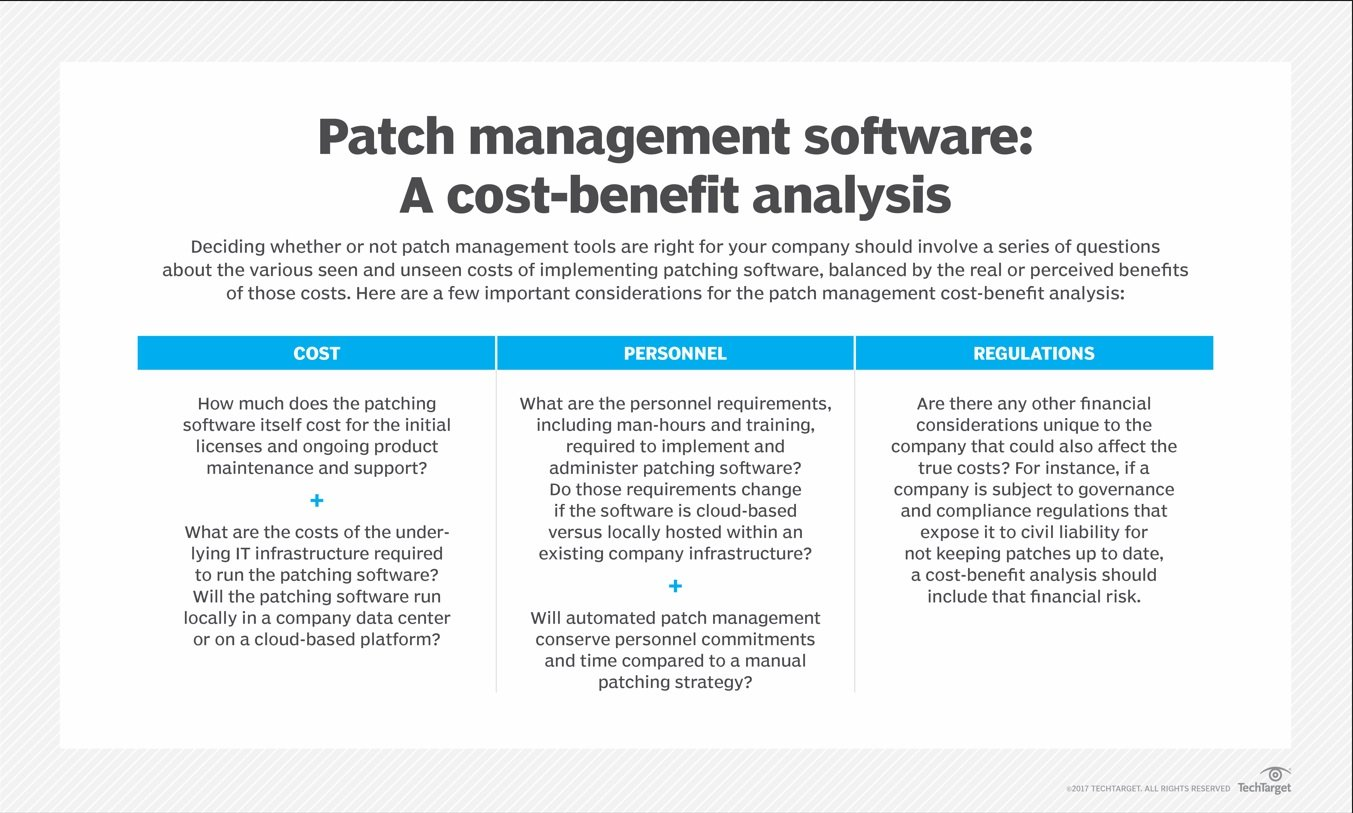
\includegraphics[width=\textwidth]{techtarget.jpg}
    \caption{Kosten baten analyse patching \autocite{Posey2024}}
    \label{fig:kostenbaten}
\end{figure}

\newpage

\section{Invloed van menselijke, technologische en organisatorische factoren op patchmanagement}

Patchmanagement binnen ERP-systemen wordt sterk beïnvloed door een combinatie van menselijke, technologische en organisatorische factoren. Een 
diepgaande analyse van deze elementen is essentieel om een effectieve patchmanagementstrategie te ontwikkelen en te implementeren. Menselijke 
factoren spelen een cruciale rol in het patchmanagementproces. Het bewustzijn van medewerkers over de noodzaak van patching en het belang van cybersecurity
is van vitaal belang. Zonder voldoende bewustwording kunnen patches over het hoofd worden gezien of niet tijdig worden toegepast, waardoor de veiligheid van het ERP-systeem in gevaar komt. Daarnaast 
is training van medewerkers essentieel om ervoor te zorgen dat ze de juiste procedures volgen bij het beoordelen, testen en implementeren van patches. 
Een goed opgeleid team kan de efficiëntie van het patchmanagementproces aanzienlijk verbeteren en de kans op menselijke fouten minimaliseren. Technologische 
factoren omvatten de beschikbaarheid en kwaliteit van patchingtools en -technologieën binnen ERP-systemen. Geavanceerde

patchingtools kunnen het patchmanagementproces automatiseren en vereenvoudigen, waardoor de werklast voor IT-teams wordt verminderd en de kans op fouten wordt verkleind. 

Het gebruik van geautomatiseerde tools kan ook zorgen voor een snellere detectie en reactie op beveiligingsdreigingen,

wat cruciaal is voor het beschermen van het ERP-systeem tegen potentiële aanvallen. Organisatorische factoren, zoals 
de samenwerking tussen verschillende afdelingen en de implementatie van duidelijke patchmanagementprocedures, zijn ook van groot belang. Een goed
 gestructureerd patchmanagementbeleid, ondersteund door heldere communicatiekanalen en duidelijke verantwoordelijkheden, kan de efficiëntie van het patchmanagementproces aanzienlijk verbeteren. Door nauw
  samen te werken met verschillende belanghebbenden, waaronderIT-teams, beveiligingsexperts en operationele afdelingen, kunnen organisaties ervoor zorgen dat patching prioriteit krijgt en effectief wordt uitgevoerd.


In het specifieke geval van SAP ERP is het belangrijk om te benadrukken dat patchmanagement niet alleen een technische kwestie is, maar ook een strategisch aspect van IT-beveiliging.

Het succesvol beheren van patches vereist daarom een holistische benadering waarbij rekening wordt gehouden met zowel menselijke, technologische als organisatorische factoren.

Door bewustwording te vergroten, medewerkers te trainen, geavanceerde tools te gebruiken en effectieve samenwerking te bevorderen, 

kunnen organisaties hun SAP ERP-systemen adequaat beschermen tegen potentiële bedreigingen en de operationele continuïteit waarborgen \autocite{Graffeo2018}.

\section{Strategieën voor minimalisering van de impact op de continuïteit}
Effectieve patching vereist zorgvuldige planning om de impact te minimaliseren. Het is raadzaam patchactiviteiten te plannen tijdens niet-kritieke operationele periodes.

Daarnaast kan een gefaseerde implementatie, beginnend met minder kritieke systemen, de operationele continuïteit waarborgen. Het implementeren van fallbackstrategieën is essentieel voor 

een snelle en efficiënte herstelprocedure in geval van onvoorziene problemen. Patching kan falen

door verschillende redenen, variërend van incompatibele hardware tot conflicten met andere patches, of een patch die goed installeert maar iets anders kapotmaakt \autocite{Shein2022}.

Het implementeren van patches binnen SAP ERP-systemen kan een aanzienlijke invloed hebben op de operationele continuïteit van een organisatie. Om deze impact te minimaliseren,

zijn er verschillende strategieën die organisaties kunnen toepassen tijdens het patchmanagementproces. Ten eerste is zorgvuldige planning essentieel, patchactiviteiten kan best gebeuren

tijdens niet-kritieke operationele periodes, zoals buiten de reguliere kantooruren of tijdens perioden van verminderde bedrijfsactiviteit. Door patches op strategische momenten toe te passen,

kan de verstoring van lopende processen tot een minimum worden beperkt. Daarnaast is een gefaseerde implementatie van patches een effectieve strategie om de impact op de continuïteit te minimaliseren. 

In plaats van alle systemen tegelijkertijd te patchen, kunnen organisaties ervoor kiezen om patches geleidelijk aan te brengen, te beginnen met

minder kritieke systemen. Op deze manier kunnen eventuele problemen of compatibiliteitsproblemen

worden geïdentificeerd en opgelost voordat de patches op cruciale systemen worden toegepast. Het opzetten van fallbackstrategieën is ook essentieel voor een succesvol patchmanagementproces.

Ondanks zorgvuldige planning en gefaseerde implementatie kunnen er onvoorziene problemen optreden tijdens het patchen, zoals systeemstoringen of conflicten tussen patches. Door fallbackstrategieën te definiëren en vooraf te plannen,

kunnen organisaties snel en efficiënt reageren op dergelijke situaties en de operationele continuïteit waarborgen. Dit kan bijvoorbeeld het creëren van back-ups van cruciale systemen omvatten, 

zodat ze snel kunnen worden hersteld in geval van problemen tijdens het patchen. In het kort benadrukken zorgvuldige planning, gefaseerde

implementatie en fallbackstrategieën het belang van een proactieve en strategische benadering van patchmanagement. Door deze strategieën

toe te passen, kunnen organisaties de impact van patchactiviteiten op de operationele continuïteit minimaliseren en tegelijkertijd de veiligheid en stabiliteit van hun SAP ERP-systemen waarborgen.

\section{Communicatiestrategieën voor belanghebbenden}
Heldere en tijdige communicatie met belanghebbenden over geplande patchactiviteiten is van vitaal belang. Het is essentieel om begrijpelijke informatie te verstrekken over de redenen achter het patchen,

mogelijke impact en benodigde voorzorgsmaatregelen \autocite{Toren2019}. Daarnaast zijn het opzetten van communicatiekanalen voor feedback en het bieden van ondersteuning aan gebruikers eveneens cruciaal voor een succesvolle implementatie.


\section{Patchmanagement in cloudgebaseerde ERP-systemen}
Volgens \textcite{Forbes2021} kan de cloud een meer gestroomlijnde benadering bieden, terwijl tegelijkertijd geprofiteerd wordt van beveiligings best practices en updates van cloud- en softwareleveranciers. Volgens \textcite{Ruiter2024} bieden

cloudgebaseerde ERP-systemen verschillende voordelen ten opzichte van traditionele on-premises oplossingen. Ze kunnen gemakkelijk de infrastructuur schalen met de groeiende behoeften van een organisatie, 

vereenvoudigen het implementatieproces van beveiligingspatches en bieden realtime zichtbaarheid in de patchstatus van alle apparaten, ongeacht hun locatie. De initiële kosten zijn lager bij de cloudinfrastructuur, en

deze kosten zijn ook meer voorspelbaar, terwijl bij een on-premise ERP-systeem de initiële kosten veel hoger kunnen zijn, maar de

totale kosten na verloop van tijd lager kunnen uitvallen, afhankelijk van de vereisten. Een ander voordeel van de cloudprovider is dat

de verantwoordelijkheid voor data beveiliging nu ook bij hen ligt. De interesse in ERP

overstijgt verticale industrieën, met fabrikanten, dienstverleners, non-profitorganisaties en overheidsentiteiten die allemaal behoefte hebben aan de mogelijkheden ervan om efficiënt en effectief te kunnen

functioneren. In de afgelopen jaren zijn velen overgestapt van decennia-oude on-premises ERP-systemen naar nieuwe cloudgebaseerde ERPs. Anderen die nooit ERP hadden, gaan rechtstreeks naar de cloudoptie, vooral 

SaaS ERP. We zien ook dat de markt dit reflecteert en dat nu minder dan een derde van de bedrijfsapplicaties naar verwachting in 2022 nog gehost zal worden op traditionele servers, terwijl de rest zal vertrouwen op cloud

computing-oplossingen. Bedrijven over de hele wereld vertrouwen nu steeds meer op cloud computing om hun bedrijf te runnen. Het groeit zo snel in populariteit dat minder dan een derde van de bedrijfsapplicaties nog verwacht wordt 

te worden gehost op traditionele servers tegen 2022, en de rest zal vertrouwen op cloud computing-oplossingen \autocite{Pimentel2017}.

Patchmanagement in cloudgebaseerde ERP-systemen is dus een steeds belangrijker wordend aspect van IT-beheer voor moderne organisaties. Met de opkomst van cloud computing hebben veel bedrijven ervoor gekozen

om hun ERP-systemen naar de cloud te verplaatsen om te profiteren van de schaalbaarheid, flexibiliteit en kosteneffectiviteit die de cloud biedt. 

Echter, het beheren van patches in een cloudomgeving brengt unieke uitdagingen met zich mee. Om succesvol patchmanagement

in cloudgebaseerde ERP-systemen te implementeren, moeten organisaties investeren in geautomatiseerde patchingtools, 

beleidsregels en procedures voor patchmanagement, en continue monitoring en rapportage van patch statussen. Daarnaast is samenwerking en communicatie tussen IT-teams, 

cloudproviders en andere belanghebbenden van vitaal belang om ervoor te zorgen dat patches tijdig worden geïmplementeerd zonder de 

operationele continuïteit te verstoren. Met de juiste aanpak kunnen organisaties de beveiliging en betrouwbaarheid van hun cloudgebaseerde ERP-systemen waarborgen in een snel evoluerend technologisch landschap.


\section{De toekomst van patchmanagement}
De toekomst van AI in patchmanagement ziet er veelbelovend uit, vooral met de groeiende uitdagingen waar organisaties mee te maken hebben bij

het beheren van patches. Elke week worden er steeds meer patches uitgebracht, wat het moeilijk maakt om te bepalen welke patches moeten worden toegepast, hoe snel dat moet gebeuren en waar. Dit zorgt voor een aanzienlijke werklast voor patchmanagementprogramma's, die nog verder toeneemt naarmate

organisaties meer eindpunten en diverse softwarebronnen toevoegen. Steeds meer bedrijven wenden zich tot AI en machine learning

om deze uitdagingen aan te pakken. Deze technologieën kunnen helpen bij het detecteren, prioriteren en snel toepassen van patches wanneer dat nodig is. Dit leidt tot een efficiëntere werking, waardoor de algehele beveiliging wordt verbeterd door kwetsbaarheden sneller te 

identificeren en de kans te verkleinen dat deze worden uitgebuit in aanvallen.

AI-algoritmen begrijpen de complexe relaties tussen verschillende variabelen en kunnen een patchschema aanbevelen dat is afgestemd op de specifieke behoeften van een organisatie. Daarnaast kunnen AI-tools compatibiliteitsrisico's 
verminderen door slimme implementatietests uit te voeren en de belasting van IT-resources te verlagen. Met AI kunnen bedrijven ook
 endpoint- en gebruikersprofielen evalueren, zodat alleen relevante patches op het juiste moment worden toegepast, met minimale impact op gebruikers en bedrijfsactiviteiten. Hoewel de toepassing van AI in patchmanagement veel potentieel heeft, zijn er 
 ook uitdagingen en risico's. Het gebruik van AI in patchmanagement is nog nieuw en organisaties moeten een steile leercurve doorlopen om deze technologie effectief te implementeren. Bovendien zijn er ethische 

overwegingen bij het gebruik van AI voor autonome beslissingen over patchprioritering en -implementatie. AI is niet perfect en de voorspellingen zijn niet altijd nauwkeurig, wat kan leiden tot fouten bij het beoordelen van de impact van patches​ \autocite{OFlaherty2023}

\section{Patchmanagement best practices}
Om patchmanagement effectief te kunnen implementeren binnen een organisatie zijn bepaalde stappen noodzakelijk. Een uitgebreide beoordeling van alle 
ERP-systemen of -programma's zou voor een bedrijf zeer nuttig blijken. Dit maakt de identificatie van ontbrekende patches mogelijk op basis van hun 
ernstniveaus en zorgt ervoor dat prioriteiten kunnen worden gesteld. Vervolgens wordt de planning van patch-implementaties cruciaal: deze moeten worden 
georganiseerd zonder nadelige gevolgen voor de productiviteit van werknemers, doorgaans door afzonderlijke implementatieschema's te gebruiken voor verschillende 
afdelingen of systemen die elkaar niet hinderen. Een patchbeheerprogramma bestaat doorgaans uit tools die automatisch patches kunnen implementeren op basis 
van de beschikbaarheid van de gebruiker en de uptime van het systeem. Naast de strategieën die zijn ontwikkeld om alle programma's te patchen, zijn het 
testen van patches na de implementatie en het garanderen van een roll-back-mogelijkheid voor patches voor het geval ze problemen veroorzaken ook noodzakelijke 
stappen voor een effectief patchbeheerproces. Het is van cruciaal belang om een ​​centraal punt voor de patchbeheeroplossing te selecteren, de nadruk te leggen 
op de patches die moeten worden geïmplementeerd en op het patchproces. \autocite{ManageEngine2024}



%%%=============================================================================
%% Methodologie
%%=============================================================================

\chapter{\IfLanguageName{dutch}{Methodologie}{Methodology}}%
\label{ch:methodologie}

%% TODO: In dit hoofstuk geef je een korte toelichting over hoe je te werk bent
%% gegaan. Verdeel je onderzoek in grote fasen, en licht in elke fase toe wat
%% de doelstelling was, welke deliverables daar uit gekomen zijn, en welke
%% onderzoeksmethoden je daarbij toegepast hebt. Verantwoord waarom je
%% op deze manier te werk gegaan bent.
%% 
%% Voorbeelden van zulke fasen zijn: literatuurstudie, opstellen van een
%% requirements-analyse, opstellen long-list (bij vergelijkende studie),
%% selectie van geschikte tools (bij vergelijkende studie, "short-list"),
%% opzetten testopstelling/PoC, uitvoeren testen en verzamelen
%% van resultaten, analyse van resultaten, ...
%%
%% !!!!! LET OP !!!!!
%%
%% Het is uitdrukkelijk NIET de bedoeling dat je het grootste deel van de corpus
%% van je bachelorproef in dit hoofstuk verwerkt! Dit hoofdstuk is eerder een
%% kort overzicht van je plan van aanpak.
%%
%% Maak voor elke fase (behalve het literatuuronderzoek) een NIEUW HOOFDSTUK aan
%% en geef het een gepaste titel.


\section{Fase 1: Literatuuronderzoek}
Fase 1 omvat een grondige literatuurstudie om de huidige staat van ERP-patchmanagement bij managed service provider te doorgronden. In dit kader worden relevante bronnen ontleed, waaronder 

academische publicaties en vakliteratuur. De kern ligt op het verdiepen van het begrip binnen patchmanagement, het opsporen van bestaande procedures voor patchmanagement en de erkenning van de uitdagingen en succescomponenten. De duur van deze fase wordt geschat op drie weken.
\section{Fase 2: Casestudy}
De tweede fase omvat het uitdiepen van een specifiek geval door middel van een casestudy bij een managed service provider. De analyse zal zich richten op hoe de onderneming het patchmanagementproces beheert. Dit

proces zal schematisch in kaart worden gebracht aan de hand van een BPMN-schema. De verwachte tijdsbestek voor deze fase is vier weken.
\section{Fase 3: Interviews}
Fase 3 is bedoeld om een gedetailleerder inzicht te verwerven in de tactieken van een managed service provider in relatie tot ERP-patchmanagement. Hiertoe zullen interviews plaatsvinden met bijvoorbeeld ERP-expertisehouders. Deze 

interviews proberen te achterhalen hoe de geïnterviewde naar het proces uit Fase 2 kijkt en waar volgens de geïnterviewde verbeteringen kunnen worden doorgevoerd. De geplande duur voor deze fase is drie weken.
\section{Fase 4: Analyse van Beschikbare Tools en Praktijken}
In de vierde worden praktijken en technologieën voor ERP-patchmanagement geanalyseerd. In deze fase staan we stil bij hoe we het proces voor patchmanagement kunnen verbeteren met behulp van tools en praktijken met. De verwachte periode voor deze fase is drie weken.
\section{Fase 5: Samenvatting en Adviezen}
In de slotfase worden de resultaten van het literatuuronderzoek, de analyses, gesprekken en het casusonderzoek samengebracht. Uit deze synthese worden conclusies getrokken en specifieke adviezen geformuleerd om de effectiviteit 

van ERP-patchmanagement in organisaties te verbeteren. Het tijdsbestek voor deze fase is drie weken. \\

\begin{figure}[h]
    \centering
    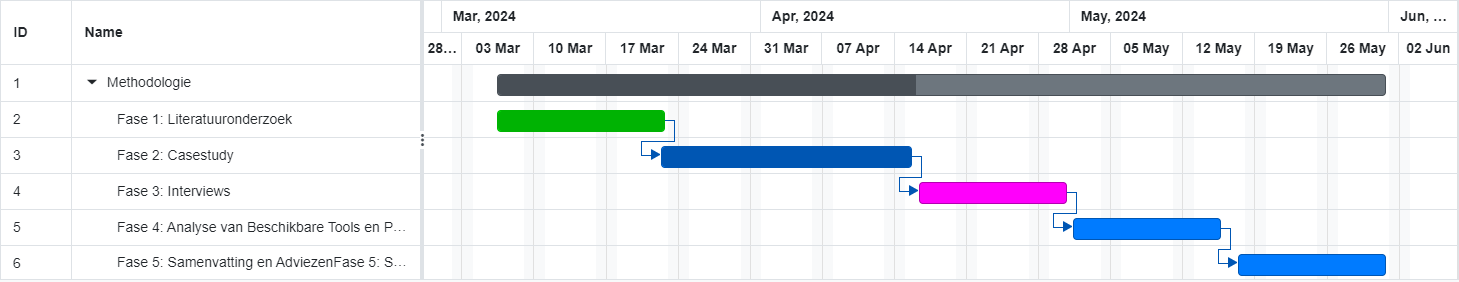
\includegraphics[width=\textwidth]{methodologie2.png}
    \caption{Schematische weergave van de methodologie}
     \label{fig:methodologie2}
\end{figure}
\newpage


% Voeg hier je eigen hoofdstukken toe die de ``corpus'' van je bachelorproef
% vormen. De structuur en titels hangen af van je eigen onderzoek. Je kan bv.
% elke fase in je onderzoek in een apart hoofdstuk bespreken.

%\input{...}
%\input{...}
%...

%%%=============================================================================
%% Conclusie
%%=============================================================================

\chapter{Conclusie}%
\label{ch:conclusie}

% TODO: Trek een duidelijke conclusie, in de vorm van een antwoord op de
% onderzoeksvra(a)g(en). Wat was jouw bijdrage aan het onderzoeksdomein en
% hoe biedt dit meerwaarde aan het vakgebied/doelgroep? 
% Reflecteer kritisch over het resultaat. In Engelse teksten wordt deze sectie
% ``Discussion'' genoemd. Had je deze uitkomst verwacht? Zijn er zaken die nog
% niet duidelijk zijn?
% Heeft het onderzoek geleid tot nieuwe vragen die uitnodigen tot verder 
%onderzoek?

Een bedrijf kan overstappen naar een cloudoplossing van een ERP-provider als het niet wil bezighouden met het patchproces.
In een case study bij een managed service provider werd onderzocht waar het patchproces verbeterd kon worden. Uit de studie bleek dat kernel patching geautomatiseerd kan worden met patchmanagementtools, waarbij specifiek naar Avantra werd gekeken. Deze tool maakt het mogelijk om het kernel patchbestand te uploaden en de patch met de juiste configuratie uit te voeren. Voor bedrijven die veel systemen beheren, kan dit een aanzienlijke tijdsbesparing opleveren, hoewel de voordelen pas op de lange termijn zichtbaar zullen zijn vanwege de tijd die nodig is om tools zoals Avantra te implementeren. Bovendien zijn dergelijke tools niet gratis, waardoor zorgvuldige overweging nodig is voordat men besluit ze in het bedrijf te integreren.
Het onderzoek biedt diepgaand inzicht in patchmanagement en benadrukt het belang van goede communicatie met belanghebbenden en het gebruik van geautomatiseerde tools voor patching. Cloudgebaseerde ERP-systemen bieden vele voordelen ten opzichte van traditionele on-premises oplossingen, zoals schaalbaarheid en kosteneffectiviteit. De toekomst van patchmanagement is veelbelovend, met de opkomst van AI en machine learning die organisaties kunnen helpen bij het efficiënter detecteren, prioriteren en communiceren met belanghebbenden. Hoewel het gebruik van AI veelbelovend is, zijn er ook uitdagingen, zoals de implementatie en ethische overwegingen.
Het implementeren van best practices, zoals het houden van een overzicht van systemen en het testen van patches voor implementatie, is essentieel voor een effectief patchmanagementproces. Dit onderzoek heeft belangrijke gevolgen voor de praktijk, omdat het laat zien hoe bedrijven patches kunnen uitvoeren die de betrouwbaarheid van hun ERP-systemen kunnen garanderen door ze sneller uit te voeren. De aanbevelingen stellen dat IT-teams, cloudproviders en andere belanghebbenden samen moeten werken en communiceren. Ze benadrukken ook de mogelijke noodzaak om te investeren in geautomatiseerde patchingtools voor regelmatig patchmanagement.



%---------- Bijlagen -----------------------------------------------------------

\appendix

\chapter{Onderzoeksvoorstel}

Het onderwerp van deze bachelorproef is gebaseerd op een onderzoeksvoorstel dat vooraf werd beoordeeld door de promotor. Dat voorstel is opgenomen in deze bijlage.

%% TODO: 
%\section*{Samenvatting}

% Kopieer en plak hier de samenvatting (abstract) van je onderzoeksvoorstel.

% Verwijzing naar het bestand met de inhoud van het onderzoeksvoorstel
%%---------- Inleiding ---------------------------------------------------------

\section{Introductie}%
\label{sec:introductie}
\usepackage{graphicx}
Dit onderzoek richt zich op het optimaliseren van het patchmanagement in groot- en middelgrote bedrijven die gebruikmaken van SAP ERP-systemen. ERP-software speelt een essentiële rol in bedrijfsomgevingen, geïllustreerd door het brede gebruik ervan, waarbij 62\% van de ondernemingen met minstens 10 werknemers in 2021 ERP-software implementeerde, volgens recente gegevens \autocite{StatistiekVlaanderen2022}.

De doelgroep van dit onderzoek bestaat uit IT-professionals en organisaties die gebruikmaken van SAP ERP-systemen, met een focus op groot- en middelgrote bedrijven. In plaats van een algemene benadering, zullen we ons concentreren op een specifieke probleemsituatie binnen deze doelgroep. Het onderwerp wordt nauwkeurig afgebakend om vanuit een casus een concrete oplossing te bieden, in lijn met het toegepaste karakter van een bachelorproef.

De probleemstelling komt voort uit de uitdagingen waarmee organisaties worden geconfronteerd bij het effectief beheren van ERP-downtime en het toepassen van patches in SAP ERP-systemen. Trage updates, compatibiliteitsproblemen en mogelijke verstoring van bedrijfsactiviteiten zijn enkele van de veelvoorkomende obstakels in het patchmanagementproces. De noodzaak om patches tijdig toe te passen, met name voor het aanpakken van beveiligingskwetsbaarheden, wordt nog verder geaccentueerd door de alarmerende toename van ransomware-aanvallen, zoals blijkt uit het feit dat alleen al in 2021 623,3 miljoen van dergelijke aanvallen werden geregistreerd \autocite{Griffiths2022}.

De centrale onderzoeksvraag van dit onderzoek luidt: "Hoe kan het patchmanagement van ERP-systemen geoptimaliseerd worden in groot- en middelgrote bedrijven die gebruikmaken van SAP ERP?" Het doel van dit onderzoek is het ontwikkelen van een holistisch begrip van de bestaande patchmanagementpraktijken, de invloed van trends in SAP ERP, en de keuze tussen handmatig en automatisch patchen. 

De onderzoeksdoelstelling is het bieden van concrete inzichten die zullen resulteren in conclusies en aanbevelingen om het ERP- patchmanagement te optimaliseren. Het verwachte eindresultaat is niet alleen een uitgeschreven scriptie, maar ook een praktisch toepasbaar resultaat zoals een rapport met aanbevelingen voor het specifieke bedrijf dat als casus dient. Het succes van dit onderzoek wordt gemeten aan de hand van de effectiviteit van de voorgestelde optimalisatiemaatregelen en de implementeerbaarheid van de aanbevelingen in de bedrijfscontext.

\subsection{Deelvragen}
- Wat zijn de bestaande patchmanagementpraktijken in groot- en middelgrote bedrijven? \\
- Welke uitdagingen en succesfactoren worden geïdentificeerd in het huidige patchmanagementproces? \\
- Wat zijn de belangrijkste trends en ontwikkelingen in SAP ERP en patchmanagement? \\
- Hoe worden opkomende technologische trends zoals cloud computing en IoT verwacht invloed te hebben op patchmanagement? \\
- Hoe beïnvloeden menselijke, technologische en organisatorische factoren de efficiëntie van patchmanagement? \\
- Welke strategieën kunnen worden toegepast om de impact op de operationele continuïteit te minimaliseren? \\
- Welke communicatiestrategieën zijn essentieel voor het informeren van belanghebbenden over patchingactiviteiten? \\

\section{State-of-the-art}%
\label{sec:state-of-the-art}

\subsection{ERP Integratie}
Het domein van ERP-downtime en patchmanagement binnen SAP ERP-systemen is complex en dynamisch, met een voortdurende evolutie van technologieën en bedrijfsbehoeften. In een studie van \autocite{StatistiekVlaanderen2022} wordt de enorme integratie van ERP-software in bedrijfsomgevingen in België benadrukt, waaruit blijkt dat 62 \% van de ondernemingen met minstens 10 werknemers in 2021 ERP-software gebruikte. Deze statistiek geeft aan dat ERP-software, die zorgt voor een geautomatiseerde gegevensuitwisseling tussen verschillende afdelingen, een essentieel instrument is geworden voor het delen van informatie binnen bedrijven. Bovendien blijkt uit de gegevens dat grotere ondernemingen vaker gebruik maken van ERP-software, waarbij maar liefst 92\% van de ondernemingen met minstens 250 werknemers deze technologie implementeerde.

\subsection{Bestaande Patchmanagementpraktijken}

In middelgrote en grote bedrijven variëren de manieren waarop ze patches beheren. Meestal betekent dit dat ze regelmatig hun software bijwerken om beveiligingsproblemen op te lossen en de prestaties te verbeteren. Toch komen ze ook voor uitdagingen, zoals langzame updates, problemen met compatibiliteit en verstoring van bedrijfsactiviteiten.

Om dit goed te doen, moeten bedrijven slimme strategieën toepassen. Een actieve aanpak, automatische patchtools en duidelijke communicatie zijn sleutels tot succes. Door vooruit te denken, automatisch te updaten en goed te communiceren met alle betrokkenen, kunnen bedrijven volgens \autocite{Firch2023} de obstakels van patchmanagement succesvol overwinnen. 

Bedrijven zijn in toenemende mate afhankelijk van ERP-systemen voor cruciale bedrijfsprocessen, waardoor de druk om downtime te minimaliseren toeneemt.
\subsection{Nood aan ERP patching }
Belangrijke softwarebedrijven brengen regelmatig patches uit met drie hoofddoelen: het aanpakken van beveiligingskwetsbaarheden, het repareren van bugs en het introduceren van nieuwe functies. Het tijdig toepassen van beveiligingspatches is cruciaal, aangezien hackers actief op zoek zijn naar kwetsbare systemen. Volgens \autocite{Griffiths2022} werden in 2021 alleen al 623,3 miljoen ransomware-aanvallen geregistreerd, een veelgebruikte tactiek bij SAP-gerelateerde aanvallen. Dit onderstreept de voortdurende noodzaak om up-to-date te blijven met de nieuwste updates. Ten tweede kunnen patches bugs repareren, waardoor de stabiliteit van de software verbetert en vervelende problemen worden geëlimineerd. Tot slot brengen leveranciers af en toe patches uit om nieuwe functies te introduceren. Deze voortdurende behoefte aan ERP-patching onderstreept het belang van effectief patchmanagement om de beveiliging, stabiliteit en functionaliteit van ERP-systemen te waarborgen.

In de huidige trends binnen SAP ERP zien we regelmatige updates die zowel de functionaliteit als de beveiliging verbeteren. Patchmanagement evolueert naar meer geautomatiseerde processen \autocite{Mukkamala2022}, waardoor bedrijven sneller en efficiënter kunnen reageren op nieuwe patches. De opkomst van cloud computing en Internet of Things (IoT) kan echter de complexiteit van patchmanagement vergroten, met nieuwe uitdagingen op het gebied van connectiviteit en beveiliging. Het is van cruciaal belang dat organisaties zich bewust zijn van deze trends en zich aanpassen aan een dynamisch ERP-landschap. 

\subsection{Manueel of Automatisch patchen}
Patchmanagementmethoden kunnen verschillende voor- en nadelen met zich meebrengen, afhankelijk van de gekozen aanpak.

Enerzijds biedt handmatig patchen meer controle aan IT-teams, waardoor ze unieke eisen kunnen accommoderen en compatibiliteitsproblemen kunnen vermijden. Deze methode maakt ook een grondige beoordeling en goedkeuring van patches mogelijk, waardoor het risico op onbedoelde gevolgen wordt verminderd.

Anderzijds is handmatig patchen tijdsintensief, waarbij voortdurende inspanningen vereist zijn om patches te monitoren, beoordelen en implementeren. De menselijke factor verhoogt bovendien het risico op fouten, en de constante monitoring van beveiligingsbulletins en patchreleases kan uitdagend zijn voor organisaties met beperkte middelen of complexe IT-infrastructuur. Automatisch patchen daarentegen biedt efficiëntie door het stroomlijnen van het patchmanagementproces en het verminderen van de werklast voor IT-teams. Het zorgt voor consistentie door patches uniform te implementeren op alle systemen, waardoor het risico op gemiste patches en kwetsbaarheden wordt verminderd. Daarnaast garandeert het een tijdige implementatie door automatisch downloaden, testen en implementeren volgens een vooraf bepaald schema.

Aan de andere kant vereist automatisch patchen een betrouwbare tool voor effectiviteit. Finetunen kan nodig zijn om problematische patches te vermijden, wat pre-implementatietests en aangepaste instellingen inhoudt. Er bestaat ook het risico van het implementeren van incompatibele patches die systeemproblemen of conflicten kunnen veroorzaken, wat regelmatige controle van patchimplementatielogs noodzakelijk maakt. Het kiezen tussen handmatig en automatisch patchen hangt af van de specifieke behoeften en middelen van een organisatie \autocite{Firch2023}. Het is dus belangrijk dat een organisatie goed beslist of ze handmatig of automatisch willen patchen, afhankelijk van hun behoeften.

\subsection{ Invloed van Menselijke, Technologische en Organisatorische Factoren}
Voor succesvol patchmanagement spelen verschillende factoren een cruciale rol. Bewustwording en training zijn essentieel voor menselijke betrokkenheid, terwijl geavanceerde patchingtools en automatisering de technologische efficiëntie verbeteren. Volgens \autocite{ServiceNow2020} bedraagt de gemiddelde tijd die nodig is om een kritieke kwetsbaarheid te patchen ongeveer 16 dagen.

Het is dus belangrijk dat organisatorische factoren, zoals een helder patchbeleid en samenwerking tussen IT-teams, de basis leggen voor een gestroomlijnd en effectief patchmanagementproces om de kwetsbaarheid zo snel mogelijk op te lossen. Samengevoegd dragen deze elementen bij aan een veilige en efficiënte IT-infrastructuur.

\subsection{ Strategieën voor Minimale Impact op Continuïteit}

Effectieve patching vereist zorgvuldige planning om de impact te minimaliseren. Het is raadzaam patchactiviteiten te plannen tijdens niet-kritieke operationele periodes. Daarnaast kan een gefaseerde implementatie, beginnend met minder kritieke systemen, de operationele continuïteit waarborgen. Het implementeren van fallback-strategieën is essentieel voor een snelle en efficiënte herstelprocedure in geval van onvoorziene problemen. Patching kan falen door verschillende redenen, variërend van onverenigbare hardware tot conflicten met andere patches, of een patch die goed installeert maar iets anders kapotmaakt \autocite{Shein2022}.

\subsection{ Essentiële Communicatiestrategieën voor Belanghebbenden}
Heldere en tijdige communicatie met belanghebbenden over geplande patchactiviteiten is van vitaal belang. Het is essentieel om begrijpelijke informatie te verstrekken over de redenen achter patching, mogelijke impact en benodigde voorzorgsmaatregelen \autocite{Toren2019}. Daarnaast zijn het opzetten van communicatiekanalen voor feedback en het bieden van ondersteuning aan gebruikers eveneens cruciaal voor een succesvolle implementatie.


\subsection{Open Vragen en Onderzoeksnoden}

Binnen het domein van ERP-patching blijven enkele wezenlijke vragen onbeantwoord. Het vinden van een optimale balans tussen het minimaliseren van operationele kosten en het beperken van schadekosten door beveiligingskwetsbaarheden vereist verdere verkenning, met specifieke aandacht voor praktische implementatieaspecten. Ook is het noodzakelijk om de impact van patchmanagement op bedrijfscontinuïteit te onderzoeken en te begrijpen hoe verschillende patchmanagementpraktijken de dagelijkse operaties van organisaties beïnvloeden. Daarnaast is er behoefte aan inzicht in hoe bedrijven van verschillende omvang ERP-systemen implementeren en welke specifieke noden zij hebben op het gebied van patchmanagement. Het onderzoek moet ook de rol van menselijke, technologische en organisatorische factoren in het ERP- patchingproces verkennen. Identificatie van de invloed van deze factoren op de efficiëntie van patchmanagement en het ontwikkelen van strategieën om hiermee om te gaan, zijn van vitaal belang om een optimaal patchmanagement te realiseren. Ten slotte moet de studie uitbreiden naar communicatiestrategieën en belanghebbendenbetrokkenheid om te begrijpen hoe effectieve communicatie kan bijdragen aan het succesvol implementeren van patchmanagementprocessen in organisaties. \\ Kortom, verdere verkenning is nodig voor een diepgaand begrip en praktische toepasbaarheid van effectief ERP-patchmanagement.
\subsection{Vergelijkbaar Onderzoek en Verschillen}

Vergelijkbare onderzoeken hebben zich gericht op aspecten van patchmanagement, maar dit voorstel onderscheidt zich door zijn holistische benadering. Waar eerdere studies zich mogelijk concentreerden op specifieke technologische trends of beveiligingsaspecten, beoogt dit onderzoek een diepgaande analyse van zowel huidige praktijken als toekomstige behoeften, met het oog op concrete efficiëntie verhogende maatregelen.

In samenvatting benadrukt de huidige literatuurstudie het belang van een gedegen begrip van patchmanagement in ERP-systemen, waarbij de nadruk ligt op de noodzaak tot optimalisatie en efficiëntieverbetering. De voorgestelde bachelorproef zal voortbouwen op deze inzichten en nieuwe bijdragen leveren aan het domein door middel van een uitgebreide analyse van praktijken, behoeften en maatregelen in groot- en middelgrote bedrijven.

%---------- Methodologie ------------------------------------------------------
\section{Methodologie}%
\label{sec:methodologie}

\subsection{Fase 1: Literatuurstudie}

In de eerste fase wordt een grondige literatuurstudie uitgevoerd om een diepgaand begrip te verkrijgen van de huidige stand van zaken in ERP-patchmanagement. Hierbij worden relevante bronnen geanalyseerd, waaronder wetenschappelijke artikelen en vakpublicaties. De focus ligt op het identificeren van bestaande patchmanagementpraktijken, uitdagingen, en succesfactoren. Deze fase zal naar verwachting twee weken in beslag nemen.

\subsection{Fase 2: Analyse van Beschikbare Tools en Technologieën}

Na de literatuurstudie volgt een analyse van beschikbare tools en technologieën voor ERP- patchmanagement. Dit omvat een evaluatie van bestaande softwareoplossingen, frameworks en technologische trends die relevant zijn voor het optimaliseren van patchprocessen. De resultaten zullen worden gebruikt om inzicht te krijgen in de technologische mogelijkheden en beperkingen. Deze fase wordt geschat op drie weken.

\subsection{Fase 3: Interviews}

Om een dieper inzicht te verkrijgen in de praktijken van groot- en middelgrote bedrijven op het gebied van ERP-patchmanagement, zullen interviews worden afgenomen bij relevante belanghebbenden, zoals IT-beheerders, security-experts en ERP-specialisten. De interviews zullen vragen bevatten om de huidige praktijken, uitdagingen en verwachtingen te achterhalen. Deze vragen zullen opgesteld worden met de opgedane kennis van voorafgaande fasen. De benodigde tijd hiervoor wordt ingeschat op drie weken.

\subsection{Fase 4: Case Studies}

Om de verzamelde informatie te valideren en specifieke situaties te begrijpen, zullen meerdere case studies worden uitgevoerd bij geselecteerde bedrijven. Hierbij worden de geïdentificeerde efficiëntie verhogende maatregelen geëvalueerd. De case studies bieden praktische inzichten en dienen als basis voor conclusies en aanbevelingen. Deze fase zal ongeveer drie weken in beslag nemen.

\subsection{Fase 5: Conclusie en Aanbevelingen}

In de laatste fase worden de bevindingen van de literatuurstudie, analyses, interviews en case studies samengebracht. Op basis hiervan worden conclusies getrokken en worden concrete aanbevelingen geformuleerd voor het optimaliseren van ERP-patchmanagement in groot- en middelgrote bedrijven. Deze fase wordt geschat op één week.

\begin{figure}
    \centering
    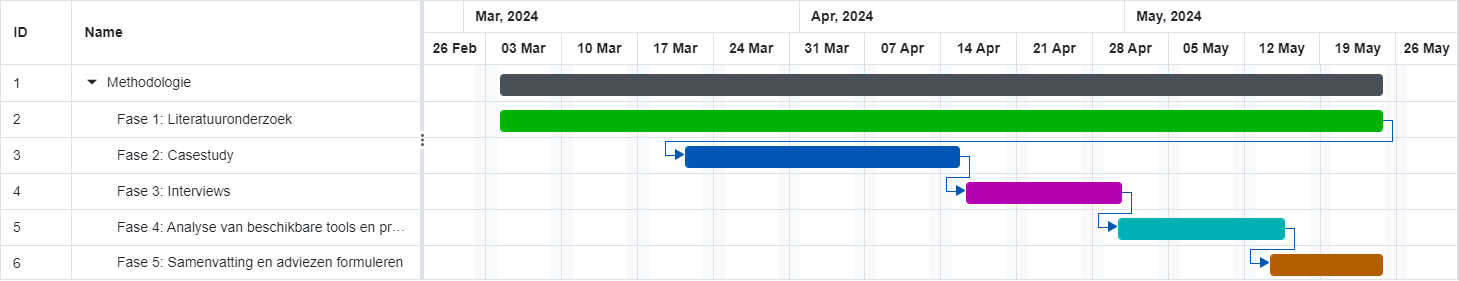
\includegraphics[width=0.5\textwidth]{methodologie.png}
    \caption{Methodologie Flowchart}
    \label{Methodologie Flowchart}
\end{figure}



%---------- Verwachte resultaten ----------------------------------------------
\section{Verwachte Resultaten en Conclusie}%
\label{sec:verwachte-resultaten}

In de complexe wereld van ERP-downtime en patchmanagement in SAP ERP-systemen, spelen groot- en middelgrote bedrijven een cruciale rol in het handhaven van operationele efficiëntie te midden van technologische evoluties. De integratie van ERP-software is wijdverbreid en daarom ook vaak een doel van cyberaanvallen, hierdoor is er nood aan het tijdig patchen van beveiligingsrisico’s. 
Patchmanagementpraktijken variëren in organisatie tot organisatie, met enkele uitdagingen zoals trage updates en compatibiliteitsproblemen. Succes hangt af van factoren zoals proactieve benaderingen, geautomatiseerde tools en heldere communicatie.
Trends in SAP ERP wijzen op regelmatige updates en een verschuiving naar geautomatiseerde patchprocessen. Menselijke, technologische en organisatorische factoren blijken cruciaal in patchmanagement. Bewustwording, training, geavanceerde tools en samenwerking zijn sleutels tot succes. Aanbevelingen omvatten strategieën voor minimale impact op de continuïteit, effectieve communicatie en het verkennen van onbeantwoorde vragen in ERP-patching.
De voorgestelde bachelorproef onderscheidt zich door zijn holistische aanpak, die waardevolle inzichten en aanbevelingen belooft voor het optimaliseren van ERP-patchmanagement in groot- en middelgrote bedrijven.


%%---------- Andere bijlagen --------------------------------------------------
% TODO: Voeg hier eventuele andere bijlagen toe. Bv. als je deze BP voor de
% tweede keer indient, een overzicht van de verbeteringen t.o.v. het origineel.
%\input{...}

%%---------- Backmatter, referentielijst ---------------------------------------

\backmatter{}

\setlength\bibitemsep{2pt} %% Add Some space between the bibliograpy entries
\printbibliography[heading=bibintoc]

\end{document}
